\documentclass[
    fontsize=12pt,              % default font size 12pt
    paper=a4,                   % DIN A4 page format
    numbers=noenddot,           % remove dots behind chapter numbers (e.g. 1.5 not 1.5.)
    listof=totoc,               % add list of figures, tables, etc. to ToC
    listof=entryprefix,         % add entry name to figures, tables, etc.
    listof=nochaptergap,        % no chapter gap for figures, tables, etc.
    bibliography=totoc,         % add bibliography to ToC but without a chapter number
    parskip=half                % half line spacing between paragraphs
]{article}

% ##################################################
% ENCODING
% ##################################################
\usepackage{cmap}               % PDF character encoding
\usepackage[T1]{fontenc}        % 8-bit font encoding
\usepackage[utf8]{inputenc}     % UTF-8 input encoding

% ##################################################
% LANGUAGE
% ##################################################
\usepackage[ngerman]{babel} % Uncomment this if you write in German
\usepackage{csquotes}         % Package for better quotations
\hyphenation{}                % Here you can define custom hyphenations
\usepackage{blindtext}        % This package can usually be deleted as this is only used to display some blindtext

% ##################################################
% DOCUMENT VARIABLES
% ##################################################
% Personal data
\newcommand{\docAuthor}{Oliver Kusch}
\newcommand{\docMatriculationNumber}{268513}
\newcommand{\docStudyProgram}{Medieninformatik Master}
\newcommand{\docStudyFaculty}{Digitale Medien}
\newcommand{\docStudyDegree}{Master}
\newcommand{\docStreetName}{Erbsenlachen 6}
\newcommand{\docPostalCode}{78050}
\newcommand{\docCity}{Villingen-Schwenningen}
\newcommand{\docEmail}{oliver.kusch@hs-furtwangen.de}

% Document data
\newcommand{\docTitle}{Entwicklung einer Augmented Reality App zur Visualisierung historischer Gebäude der Stadt Villingen} % This is the main title of this document (thesis)
\newcommand{\docSubTitle}{}            % leave empty to remove
\newcommand{\docType}{Thesis}                            % Usually this will be 'Thesis"
\newcommand{\docSupervisor}{Prof. Dr. Uwe Hahne}             % Your supervisor
\newcommand{\docCoSupervisor}{Prof. Dr. Thomas Schneider}        % Your co-supervisor
\newcommand{\docDeadline}{31.08.2022}                      % This is the date when you submit the document

% ##################################################
% BIBLIOGRAPHY 
% ##################################################
\usepackage[backend=bibtex]{biblatex}
\addbibresource{literatur/library.bib}

\usepackage[acronym, toc, nogroupskip, nopostdot, nonumberlist]{glossaries}
\usepackage[acronym]{glossaries}
%\makeglossaries

%Acronym AR und Tracking
\newacronym{ar}{AR}{Augmented Reality}
\newacronym[]{vr}{VR}{Virtual Reality}
\newacronym[]{mr}{MR}{Mixed Reality}
\newacronym[]{ve}{VE}{Virtual Environments}
\newacronym[]{imu}{IMU}{Inertial Measurement Units}
\newacronym[]{dof}{DOF}{Degrees of Freedom}
\newacronym[]{fast}{FAST}{Features from accelerated segment test}
\newacronym[]{sift}{SIFT}{Scale Invariant Feature Transform}
\newacronym[]{surf}{SURF}{Speeded Up Robust Features}
\newacronym[]{orb}{ORB}{Oriented Fast and Rotated Brief}
\newacronym{slam}{SLAM}{Simultaneous Localization and Mapping}
\newacronym{ptam}{PTAM}{Parallel Tracking and Mapping}
\newacronym{uml}{UML}{Unified Modeling Language}
\newacronym{rest}{REST}{Respresentational State Transfer}
\newacronym{json}{JSON}{JavaScript Object Notation}

%Acronyms App
\newacronym{sdk}{SDK}{Software Develpoment Kit}

\newacronym{Materials}{Materials}{Materials affektieren das Aussehen eines 3D Objekts mit einer oder mehrerer Texturen, Farben oder den Eigenschaften von Reflexionen}
\newacronym{grafik-rendering-pipeline}{GRP}{Grafik-Rendering-Pipeline}
\newacronym{frames-per-second}{FPS}{Frames Pro Sekunde}
\newacronym{cpu}{CPU}{Central Processing Unit}
\newacronym{gpu}{GPU}{Graphics Processing Unit}

\makenoidxglossaries


% ##################################################
% PDF SETTINGS
% ##################################################
\usepackage[
    colorlinks=true,
    linkcolor=black,
    citecolor=black,
    filecolor=black,
    urlcolor=black,
    bookmarks=true,
    bookmarksopen=true,
    bookmarksopenlevel=3,
    bookmarksnumbered,
    plainpages=false,
    pdfpagelabels=true,
    hyperfootnotes,
    pdftitle ={\docTitle},
    pdfauthor={\docAuthor},
    pdfcreator={\docAuthor}
]{hyperref}

% ##################################################
% FONTS AND SPACING
% ##################################################

\renewcommand{\baselinestretch}{1.5} % default 1.5 spacing
\raggedbottom                        % don't stretch spacing to fit page length
\usepackage{lmodern}                 % Allow font sizes at arbitrary sizes
\usepackage{microtype}               % Bessere Worttrennung. Wirkt overful hbox entgegen
\usepackage{textgreek}               % Allow alpha, beat, gamma ... in text without Mathmode

% ##################################################
% PAGE FORMATTING
% ##################################################
% Page layout, see http://mirrors.ctan.org/macros/latex/contrib/geometry/geometry.pdf #3 Page geometry
\usepackage[
    bindingoffset=1.5cm, % Specify an offset if you plan to bind the document
    inner=2.5cm,         % Left Spacing
    outer=2.5cm,         % Right spacing
    top=3cm,             % Top spacing
    bottom=2cm,          % Bottom spacing
    twoside              % Delete this if you don't want to use double-sided pages
]{geometry}

% Page header
\usepackage{fancyhdr}
\fancypagestyle{scrheadings}
{
  \fancyhead[EL]{\thepage}% gerade Seiten, links
  \fancyhead[ER]{\nouppercase{\leftmark}}% gerade Seiten, rechts
  \fancyhead[OL]{\nouppercase{\leftmark}}% ungerade Seiten, links
  \fancyhead[OR]{\thepage}% ungerade Seiten, rechts
  \fancyfoot[C]{}
}
\setlength{\headheight}{18pt}           % set headheight to 18pt
\addtolength{\skip\footins}{0.5cm}      % spacing at the end of page (footnotes)

%\usepackage[
 %   headsepline,                        % seperator line beneath page header on normal pages
 %   plainheadsepline                    % seperator line beneath page header on pages like ToC
%]{scrlayer-scrpage}
%\clearpairofpagestyles                  % clear default settings
%\addtokomafont{pagehead}{\normalfont}   % use normal font for page header
%\ohead*{\thepage}                       % page number
%\ihead{\headmark}                       % chapter name
%\automark[section]{section}             


\usepackage[bottom]{footmisc}           % Always place footer at end of page

\usepackage{multicol}                   % Format text in multiple columns
\usepackage{emptypage}                  % Support for empty pages via \cleardoublepage
\usepackage{lscape}                     % Support for landscape pages
\usepackage{titlesec}
\usepackage{hyperref}

\titleclass{\subsubsubsection}{straight}[\subsection]

\newcounter{subsubsubsection}[subsubsection]
\renewcommand\thesubsubsubsection{\thesubsubsection.\arabic{subsubsubsection}}
\renewcommand\theparagraph{\thesubsubsubsection.\arabic{paragraph}} % optional; useful if paragraphs are to be numbered

\titleformat{\subsubsubsection}
  {\normalfont\normalsize\bfseries}{\thesubsubsubsection}{1em}{}
\titlespacing*{\subsubsubsection}
{0pt}{3.25ex plus 1ex minus .2ex}{1.5ex plus .2ex}

\makeatletter
\renewcommand\paragraph{\@startsection{paragraph}{5}{\z@}%
  {3.25ex \@plus1ex \@minus.2ex}%
  {-1em}%
  {\normalfont\normalsize\bfseries}}
\renewcommand\subparagraph{\@startsection{subparagraph}{6}{\parindent}%
  {3.25ex \@plus1ex \@minus .2ex}%
  {-1em}%
  {\normalfont\normalsize\bfseries}}
\def\toclevel@subsubsubsection{4}
\def\toclevel@paragraph{5}
\def\toclevel@paragraph{6}
\def\l@subsubsubsection{\@dottedtocline{4}{7em}{4em}}
\def\l@paragraph{\@dottedtocline{5}{10em}{5em}}
\def\l@subparagraph{\@dottedtocline{6}{14em}{6em}}
\makeatother

\setcounter{secnumdepth}{4}
\setcounter{tocdepth}{4}

% ##################################################
% IMAGES AND FIGURES
% ##################################################
\usepackage{graphicx}                   % support for including images
\graphicspath{{img/}}                   % default path
\usepackage{subfig}

% simple numbering without chapter
\renewcommand{\thefigure}{\arabic{figure}}

% ##################################################
% TikZ | Support for drawing diagrams
% ##################################################
\usepackage{tikz}
\usepackage{float}
\usetikzlibrary{shapes.geometric, arrows, positioning, decorations.pathreplacing, calc}
\tikzstyle{box} = [rectangle, minimum width=3cm, minimum height=1cm, text centered, draw=black, fill=orange!30]
\tikzstyle{mainbox} = [rectangle, minimum width=3cm, minimum height=1cm, text centered, draw=black, fill=green!30]
\tikzstyle{plainbox} = [rectangle, minimum width=3cm, minimum height=1cm, text centered, draw=black, fill=white,thick]
\tikzstyle{border} = [rectangle, minimum width=3cm, minimum height=1cm, text centered, draw=black]
\tikzstyle{arrow} = [thick,->,>=stealth]

\pgfdeclarelayer{foreground}
\pgfdeclarelayer{background}
\pgfsetlayers{background,main,foreground}

% ##################################################
% MATH
% ##################################################
\usepackage{amstext}
\usepackage{amsmath}

\usepackage{tabularx}
\newenvironment{conditions*}
  {\par\vspace{\abovedisplayskip}\noindent
   \tabularx{\columnwidth}{>{$}l<{$} @{${}={}$} >{\raggedright\arraybackslash}X}}
  {\endtabularx\par\vspace{\belowdisplayskip}}

% ##################################################
% SUPPORT FOR DIRECTORY TREE RENDERING
% ##################################################
\usepackage{dirtree}

% ##################################################
% SUPPORT FOR CODE LISTINGS
% ##################################################
\usepackage{listings}
\lstset{numbers=left}
\usepackage{color}
\usepackage{xcolor}

% \definecolor{backcolour}{rgb}{0.95,0.95,0.95} % Custom color for code background
% \definecolor{codegreen}{rgb}{0,0.6,0}         % Custom color for comments in your code
% \definecolor{codegray}{rgb}{0.5,0.5,0.5}      % Custom color for numbers in your code
% \definecolor{codepurple}{rgb}{0.58,0,0.82}    % Currently unused

% \renewcommand{\lstlistingname}{Code Snippet} % Here you can change the code listing name


\definecolor{codegreen}{rgb}{0,0.6,0}
\definecolor{codegray}{rgb}{0.5,0.5,0.5}
\definecolor{codepurple}{rgb}{0.58,0,0.82}
\definecolor{backcolour}{rgb}{0.95,0.95,0.92}

\lstdefinestyle{mystyle}{
    backgroundcolor=\color{backcolour},   
    commentstyle=\color{codegreen},
    keywordstyle=\color{magenta},
    numberstyle=\tiny\color{codegray},
    stringstyle=\color{codepurple},
    basicstyle=\ttfamily\footnotesize,
    breakatwhitespace=false,         
    breaklines=true,                 
    captionpos=b,                    
    keepspaces=true,                 
    numbers=left,                    
    numbersep=5pt,                  
    showspaces=false,                
    showstringspaces=false,
    showtabs=false,                  
    tabsize=2
}
\lstset{style=mystyle}

% \lstdefinestyle{normal}{
%     backgroundcolor=\color{backcolour},
%     commentstyle=\color{codegreen},
%     keywordstyle=\color{magenta},
%     numberstyle=\tiny\color{codegray},
%     stringstyle=\color{orange},
%     basicstyle=\ttfamily\small,
%     breakatwhitespace=false,
%     breaklines=true,
%     captionpos=b,
%     keepspaces=true,
%     numbers=left,
%     numbersep=5pt,
%     showspaces=false,
%     showstringspaces=false,
%     showtabs=false,
%     tabsize=2,
%     rulecolor=\color{black},
%     frame=L,
%     xleftmargin=6px
% }
% \lstset{style=normal}                % Load preamble

\begin{document}

\include{framework/titlepage}   % Title page
\addcontentsline{toc}{section}{\abstractname} % \abstractname is the default name, you can customize it
\thispagestyle{plain}
\begin{center}
    \Large
    \textbf{Abstract}
\end{center}

\noindent
Durch das Projekt NISABA\footnote{https://nisaba.dm.hs-furtwangen.de/} und der Veranstaltung Bildverarbeitung und Computergrafik im Studiengang Medieninformatik Master im Sommersemester 2021 sind 3D-Modelle der Kasernengebäude des Lyautey- und Mangin-Geländes entstanden. Um die fertigen 3D Modelle für jeden zugänglich und auf moderner Weise präsentieren zu können, wird in dieser Master-Arbeit eine Augmented Reality Anwendung für Smartphone und Tablet Geräte entwickelt.

Diese Forschungsarbeit beschäftigt sich mit der Entwicklung einer Augmented Reality \acrshort{ar} Anwendung. Durch genaues Tracking und eine realistische Darstellung der Gebäude durch wetterspezifische Belichtung, Schattierung und Spiegelung soll eine hohe Immersion erschaffen werden. In der Anwendung werden die 3D-Objekte in der Größendarstellung 1:1 über das Videobild der Kamera gelegt und der Nutzer kann vor Ort das Gebäude in Echtzeit ein- und ausblenden lassen. Dafür wird der Begriff \textit{world-scale Augmented Reality} herangezogen. Bekannte Beispiele sind das AR Spiel Pokemon GO\footnote{https://pokemongolive.com/de/} oder auch Anwendungen für Googles Holo Lens\footnote{https://www.microsoft.com/de-de/hololens}.

%Immersion in AR -> Recherche worauf kommt es an?
Eine wesentliche Rolle bei der Immersion in AR spielt das Tracking, bei dem kontinuierlich die Positions- und Rotationsdaten des Endgeräts erfasst werden.%Quelle
Es gibt mehrere Verfahren, um die Position und Orientierung der Kamera relativ zur Umgebung zu bestimmen. Im begrenzten Räumen ist das Tracking durch einheitlichere Belichtung und vorhandenen Kanten und Flächen mit kamerabasierten Tracking Methoden gut umsetzbar. Im Freien kann das Tracking je nach Umgebung Probleme bereiten. Schwierigkeiten entstehen durch unterschiedliche Lichtverhältnisse und dem größeren Suchraum. Hinzu kommt, dass durch die große Distanz zwischen Kamera und virtuellem Objekt die Platzierung des 3D-Modells bereits durch kleine Bewegung der Kamera stark von der korrekten Position abweicht. Das Objekt erscheint nicht homogen in der realen Welt, wodurch die Immersion beeinträchtigt wird.
%Was sind die Probleme bei Outdoor Augmented Reality? Recherche

Klassischerweise wird bei AR im Freien GPS und die Neigungs- und Beschleunigungssensoren der Smartphones genutzt, um die Kameraposition und -orientierung zu ermitteln. Wie Platinsky und seine Koautoren\cite{platinsky} bereits erörtert ist die GPS Lokalisierung insbesondere in Städten mit Störfaktoren wie Gebäuden oder Vegetation ungenau. Deshalb wird in dieser Arbeit auf Methoden eingegangen, um die Genauigkeit der Position und der Orientierung der Kamera im Freien zu verbessern.

Um die Immersion bei der Nutzung der App zu steigern, werden die Wetterbedingungen bei der Darstellung der 3D-Modelle berücksichtigt. So sollen die Fassaden bei regnerischem Wetter dunkler und gegebenenfalls spiegelnd dargestellt werden. Die Schattierungen sollen sich anpassen, indem bei hartem Licht (z.B. durch starke Sonneneinstrahlung) auch harte Schatten und bei weichem Licht (z.B. bei einer dichten Wolkendecke) weiche Schatten dargestellt werden.    % Abstract
\setglossarystyle{list}
\printglossary[type=\acronymtype,title=Abkürzungsverzeichnis,style=tree] % \acronymname is the default name, you can customize it

\newpage
\tableofcontents         % Table of contents
%\newacronym{ar}{AR}{Augmented Reality}

\newacronym{slam}{SLAM}{Simultaneous Localization and Mapping}     % List of figures, bibliography
%\printglossary[type=\acronymtype,title=Abkürzungsverzeichnis,toctitle=Abkürzungsverzeichis]
%\printglossary[type=\acronymtype]
\printnoidxglossary[type=\acronymtype,title=Abkürzungsverzeichis,toctitle=Abkürzungsverzeichis]
\clearpage

% KAPITEL 1 Einleitung
% Zielsetzung / Fragestellungen / Hintergrund
\section{Einleitung}
%Motivation
Durch vorangegangene Projekte sind mit photogrammetrischen Methoden 3D Modelle von historisch bedeutenden Gebäuden des SABA, des Lyautley- und des Mangin-Geländes der Stadt Villingen entstanden. Die Gebäude sind virtuell gespeichert, jedoch werden diese nicht weiter verwendet. In dieser Arbeit wird eine Augmented Reality Anwendung für Smartphones entwickelt, die eine Visualisierung der Modelle mit der AR Technologie bietet. Somit haben Bewohner der Stadt Villingen und interessierte Personen wie Touristen, die mehr über die Geschichte der Stadt Villingen erfahren möchten, zugriff auf die Modelle und können damit einen Teil der Stadtgeschichte erleben.

%Aufgabenstellung/Zielsetzung/Probleme
Die Aufgabe besteht darin eine Anwendung zu entwickeln, die zum einen die Gebäude mittels GPS vor Ort platziert. Die Gebäude werden dabei im Größenverhaltnis 1:1 dargestellt, sodass der Nutzer einen realistischen Eindruck bekommt, wie das Gebäude in Echt ausgesehen hat. Zum anderen ist es möglich die Gebäude auf jeder beliebigen horizontalen Fläche zu platzieren. Die Anwendung baut auf aktuelle AR Software Development Kits (ARCore bzw. ARKit) auf und wird mit der Game Engine Unity und AR Foundation entwickelt.

Ziel ist es eine hohe Immersion bei der Nutzung zu schaffen. Das Gebäude soll nahtlos im Kamerabild dargestellt werden. So wird eine Wetter REST-API angebunden (OpenWeatherMap), um aktuelle Wetterdaten abzurufen. Daraufhin wird die Darstellung der Modelle angepasst. Bei Regen wird die Szene dunkler, Materialien werden nass dargestellt und spiegeln die Umgebung. Herrscht starker Sonnenschein, so wird die Intensität des Lichts verändert und harte Schatten geworfen.

Diese Arbeit untersucht die Möglichkeiten von AR und dessen Limitierungen in einer freien Umgebung. Mit der GPS Funktionalität werden Genauigkeitsprobleme der GPS-Antennen in Smartphones untersucht.

In dieser Arbeit werden zunächst einleitend theoretische Grundlagen von Augmented Reality beschrieben. Auf der technischen Seite wird das Tracking, die Algorithmen zur Erkennung von Merkmalen, GPS Systeme und die Rendering Pipeline erläutert. Anschließend wird die Umsetzung der Anwendung beschrieben, indem auf das Konzept und die Implementierung der genannten Funktionalitäten eingegangen wird. Daraufhin werden bestehende Probleme und Limitierungen, die während der Entwicklung und dem Testing vorgekommen sind, veranschaulicht. Zuletzt werden Ideen für Erweiterungen und Verbesserungen der Anwendung vorgeschlagen.
\subsection{Hintergrund der Arbeit}
\subsubsection{Photogrammetrische Aufzeichnungen des SABA Geländes}
Das studentische Forschungsprojekt aus dem Wintersemester 19/20 \cite{reich2020} befasst sich mit  der Photogrammetrischen Aufzeichnung des SABA-Geländes in Villingen-Schwenningen. SABA (Schwarzwälder Apparate-Bau-Anstalt) war ein deutsches Unternehmen, das unter anderem elektronische Geräte für den Rundfunk herstellte. Der Entwicklungs- und Produktionsstandort war das Gebäude in Villingen. Aufgrund der Größe des Unternehmens (mehr als 6000 Mitarbeiter), hatte SABA eine große Bedeutung für die Stadt. 1986 wurde das Unternehmen aufgelöst, bis das Gebäude am 11. August 2021 abgerissen wurde.\footnote{https://dewiki.de/Lexikon/SABA, zuletzt aufgerufen am 17.03.2022} 

Mithilfe von Drohnen- und Bodenaufnahmen wird ein 3D Modell des SABA Geländes mit photgrammetrischen Algorithmen erzeugt. \textit{Regard3D} \footnote{https://www.regard3d.org/}, \textit{RealityCapture} \footnote{https://www.capturingreality.com/}, \textit{VisualSFM} \footnote{http://ccwu.me/vsfm/} und \textit{Meshroom} \footnote{https://github.com/alicevision/meshroom} werden im Projektverlauf genutzt und verglichen, wobei \textit{Meshroom} als kostenlose Open-Source Software hauptsächlich genutzt wird. Das Hauptgebäude wird nach der Erstellung des Meshes aus \textit{Meshroom} neu modelliert. Aufgrund der hohen Dichte der Vertices ist die Aufteilung der einzelnen Gebäude-Elemente wie Fenster, Wand und Türen schwierig. Durch eine Neumodellierung wird das Modell klarer und die Texturierung wird vereinfacht. Als Grundlage dient dabei das generierte Mesh aus \textit{Meshroom}. Als Modellierunssoftware wird \textit{Blender} benutzt.\footnote{https://www.blender.org/} In Abbildung \ref{fig:SABA3DModell} ist das fertige 3D Modell zu sehen.

\begin{figure}[ht]
    \centering
    \includegraphics[width=0.6\textwidth]{vorangegangene_Projekte/saba_modell.jpg}
    \caption{Das 3D Modell des SABA Hauptgebäudes in der 3D Karte aus den Drohnen-Aufnahmen.}
    \label{fig:SABA3DModell}
\end{figure}

\subsubsection{Photogrammetrische Aufzeichnungen des Lyautey Geländes}
Im Projekt \textit{NISABA} \cite{nisaba2021} aus dem Sommersemester 2020 und Wintersemester 2020/21 sind 3D Modelle von Gebäuden des ehemaligen Lyautey Kasernengeländes (das heutige "Richthofen") entstanden. Auch in diesem Projekt werden verschiedene Photogrammetrie Programme genutzt. \textit{Meshroom}, \textit{Pix4DMapper} \footnote{https://www.pix4d.com/de/produkt/pix4dmapper-photogrammetrie-software}, \textit{Agisoft Metashape} \footnote{https://www.agisoft.com/} und \textit{WebODM} \footnote{https://www.opendronemap.org/webodm/} weden für dieses Projekt verwendet. Gute Ergebnisse erzielt dabei \textit{Pix4DMapper}, da viele Einstellungen über den Detailgrad getroffen und mehrere Projekte kombiniert werden können. Aus dem generierten Mesh wird auch hier eine Nachmodellierung in \textit{Blender} durchgeführt.

Das Lyautey Gelände umfasst insgesamt sieben Gebäude. Für jedes Gebäude gibt es ein fertiges Modell aus \textit{Pix4DMapper} und ein Modell, bei dem die Polygone reduziert sind. Nur das Manschaftsgebäude gibt es nachmodelliert. Das ist das Gebäude 4 in der Abbildung \ref{fig:lyautey-map}. Alle 3D Modelle können auf der Website des \textit{NISABA}-Projekts \footnote{https://nisaba.villingen-schwenningen.de/uebersicht/} begutachtet werden. 

\begin{figure}[h]
    \centering
    \includegraphics[width=0.8\textwidth]{img/vorangegangene_Projekte/lyautey_map.jpg}
    \caption{Eine Übersicht der Gebäude auf dem Lyautey-Gelände.}
    \label{fig:lyautey-map}
\end{figure}

\subsubsection{Photogrammetrische Aufzeichnungen des Mangin Geländes}
Im Zuge der Veranstaltung Bildverarbeitung und Computergrafik im Sommersemester 2021 im Studiengang Medieninformatik Master sind weitere 3D Modelle entstanden\cite{kusch2021}. Die Gebäude befinden sich auf dem für die Stadt historisch wichtigen Kasernengelände Mangin in Villingen-Schwenningen, das sich direkt östlich vom Lyautey befindet. Dabei handelt es sich um ein verlassenes Kasernengelände mit architektonisch und historisch interessanten Gebäuden. Die Aufnahmen der Gebäude erfolgte in Zusammenarbeit mit dem Vermessungsamt Villingen-Schwenningen. Es wurden Aufnahmen von den Gebäuden 2-8 und 10-12 gefertigt. In der Abbildung x ist eine Übersichtskarte des Geländes mit Nummerierungen der Gebäude zu sehen.  Die Bilder aus der Luft wurden mit einer Drohne vom Vermessungsamt gemacht, während die Aufnahmen am Boden von den Studierenden aufgenommen wurden. Als Photogrammetrie-Software wird hauptsächlich \textit{Pix4DMapper} und \textit{Meshroom} verwendet. 

\begin{figure}[h]
    \centering
    \includegraphics[width=0.8\textwidth]{img/vorangegangene_Projekte/mangin_map.jpg}
    \caption{Eine Übersicht der Gebäude auf dem Mangin-Gelände.}
    \label{fig:mangin-map}
\end{figure}
\subsubsection{Übersicht vorhandener 3D Modelle}
Einige Modelle sind nicht vollständig, haben aufgrund der Vegetation vor Ort Löcher im Mesh oder einen niedrigen Detailgrad. Daher können in dieser Arbeit nicht alle 3D Modelle verwendet werden. Die Tabelle \ref{tab:uebersicht-3Dmodelle} zeigt eine Liste der vorhandenen 3D Modelle. Die Gebäude sind wie in den Übersichtskarten nummeriert. Ein geringer Detailgrad bedeutet, dass das Mesh Löcher hat oder unvollständig ist. Ein mittlerer Detailgrad zeichnet sich durch ein vollständiges Mesh mit geringen Details aus. Gebäude mit einen hohen Detailgrad können für die \Gls{ar} Anwendung genutzt werden. Händisch modellierte Gebäude haben einen sehr hohen Detailgrad.
\begin{table}[h]
    \centering
    \begin{tabular}{|p{0.1\textwidth}|p{0.25\textwidth}|p{0.04\textwidth}|p{0.15\textwidth}|p{0.1\textwidth}|p{0.17\textwidth}|}
    \hline
        Gelände & Bezeichnung                                   & Nr.   & Detailgrad    & Vertices   & Texturenanzahl   \\ \hline 
        SABA    & Karte                                         & -     & gering        & 458.311    & 1                \\ \hline
        SABA    & Hauptgebäude \newline Neumodellierung         & 1     & sehr hoch     & 44.708     & 34               \\ \hline
        SABA    & Heizwerk                                      & 2     & mittel        & 142        & 8                \\ \hline
        Lyautey & Karte                                         & -     & mittel        & 2.049.590  & 1                \\ \hline
        Lyautey & Reithalle                                     & 1     & hoch          & 1.386.531  & 1                \\ \hline
        Lyautey & Mannschaftsgebäude 1                          & 2     & hoch          & 1.255.734  & 1                \\ \hline
        Lyautey & Wirtschaftsgebäude                            & 3     & hoch          & 1.610.983  & 1                \\ \hline
        Lyautey & Mannschaftsgebäude 2                          & 4     & hoch          & 175.352    & 1                \\ \hline
        Lyautey & Mannschaftsgebäude 2 \newline Neumodellierung & 4     & sehr hoch     & 2.046      & 45               \\ \hline
        Lyautey & Stabshaus                                     & 5     & gering        & -          & -                \\ \hline
        Lyautey & Familienhaus                                  & 6     & mittel        & 119.574    & 1                \\ \hline
        Lyautey & Kammergebäude                                 & 7     & hoch          & 269.460    & 1                \\ \hline
        Mangin  & Karte                                         & 1     & mittel        & 502.040    & 1                \\ \hline
        Mangin  & Casino                                        & 2     & mittel        & 681.082    & 1                \\ \hline
        Mangin  & -                                             & 3     & hoch          & 381.633    & 1                \\ \hline
        Mangin  & Pferdestall                                   & 4     & mittel        & 242.984    & 1                \\ \hline
        Mangin  & -                                             & 6     & gering        & 500.463    & 1                \\ \hline
        Mangin  & -                                             & 7     & gering        & 31.490     & 1                \\ \hline
        Mangin  & -                                             & 8     & hoch          & 5.093      & 1                \\ \hline
        Mangin  & -                                             & 10    & hoch          & 500.307    & 1                \\ \hline
        Mangin  & -                                             & 11    & mittel        & 427.753    & 1                \\ \hline
        Mangin  & -                                             & 12    & mittel        & 497.625    & 1                \\ \hline
        Mangin  & -                                             & 17    & gering        & 5.179      & 1                \\ \hline
        Mangin  & -                                             & 23    & gering        & 998        & 1                \\ \hline
        Mangin  & Karte der Gebäude 17-23                       & -     & mittel        & 15.433     & 1                \\ \hline
    \end{tabular}
    \caption{Eine Übersicht der vorhandenen 3D Modelle.}
    \label{tab:uebersicht-3Dmodelle}
\end{table}



% KAPITEL 2 Theoretische Grundlagen / Forschungsstand
% WICHTIG: Warum braucht der leser die Informationen, um die Arbeit zu verstehen?
% Einordnung AR
\section{Theoretische Grundlagen}
\subsection {Einordnung VR, AR und MR}
%Was ist AR
Bei Augmented Reality (\acrshort{ar}) Anwendungen werden dreidimensionale virtuelle Objekte in eine echte dreidimensionale Umgebung in Echtzeit integriert. Es handelt sich um eine Variation der Virtual Environments (\acrshort{ve}), der Virtuellen Realität (\acrshort{vr}) \cite{Azuma1997}. Gerne wird zwischen \acrshort{ar}, \acrshort{vr} und Mixed Reality (\acrshort{mr}) unterschieden. Speicher und seine Ko-Autoren \cite*{Speicher2019} haben zur Eingrenzung Charakteristiken definiert, die aus Interviews mit Experten hervorgehen. 

%VR
\acrshort{vr} hat die Eigenschaft eine komplett synthetisch generierte, virtuelle Welt darzustellen. So bietet sich die Möglichkeit für den Nutzer unerreichbare Orte zu erleben. Es werden hierfür VR-Headsets wie die Oculus Rift S\footnote{https://www.oculus.com/rift-s/, zuletzt aufgerufen am 27.07.2022} oder die Playstation VR\footnote{https://www.playstation.com/de-de/ps-vr/, zuletzt aufgerufen am 27.07.2022} benötigt und die Bewegung des Headsets muss getrackt\footnote{siehe Kapitel \ref{tracking} \nameref{tracking}} werden. Der Nutzer ist während der VR-Erfahrung von der echten Umgebung isoliert, wodurch die soziale Interaktion gering ist. 

%AR
Zusätzlich zu der Definition Azumas\cite{Azuma1997} von \acrshort{ar} wird die Eigenschaft genannt, dass der virtuelle Content dazu in der Lage ist mit der echten Welt zu interagieren. Im Gegensatz zu \acrshort{vr} ist der Nutzer im gegenwärtigen physischen Raum gebunden. Die menschliche Wahrnehmung wird durch das augmentieren und der Kreation von Content Erfahrungen verbessert\cite{Speicher2019}.

%MR
Die Eingrenzung von \acrshort{mr} ist nicht eindeutig. So wird \acrshort{mr} als Kombination von AR und VR gesehen. Die Anwendungen bieten die Möglichkeit sowohl AR als auch VR zu nutzen. Auch wird Mixed Reality in Verbindung mit spezifischer Hardware wie die HoloLens\footnote{https://www.microsoft.com/de-de/hololens, zuletzt aufgerufen am 27.07.2022} gebracht. Ein weiteres Beispiel ist Pokemon GO\footnote{https://pokemongolive.com/de/, zuletzt aufgerufen am 27.07.2022}, bei dem zwischen der AR Funktion und einer virtuellen Umgebung umgeschaltet werden kann.

In Abbidldung \ref*{fig: RV_Kontinuum} haben Milgram und seine Ko-Autoren eine Grafik definiert, die das \textit{Reality-Virtuality Continuum} darstellt. Die linke Hälfte des Kontinuums repräsentiert jede Umgebung, die rein aus realen Objekten besteht, persönlich betrachtet wird und durch jegliche Art wie den Blick durch ein Fenster oder eines Displays erweitert wird. Die rechte Hälfte besteht aus rein virtuellen Objekten, die entweder Monitor-basierend oder immersiv sind. Durch diese Darstellung wird \acrshort{mr} zwischen diesen beiden Extremen eingeordnet und als Umgebung definiert, die die reale und die virtuelle Welt zusammen in einem Display darstellt \cite{Milgram1995}.

\begin{figure}[H]
    \centering
    \includegraphics[width=\textwidth]{img/einordnung_vr_ar_mr/vr_ar_mr_kontinuum.jpg}
    \caption{Das Reality-Virtuality Kontinuum nach Milgram\cite{Milgram1995}.}
    \label{fig: RV_Kontinuum}
\end{figure}

Nach diesen Definitionen wird die Anwendung dieser Arbeit in die Augmented Reality eingeordnet. Die virtuellen Objekte in Form der Gebäude werden in die echte dreidimensionale Welt projiziert. Der Nutzer hat die Möglichkeit mit diesen zu interagieren. Jedoch wird es nicht möglich sein den betrachteten Raum zu verlassen und in eine reine virtuelle Welt umzusteigen. 

% Technische Grundlagen
\subsection{Tracking}
\label{tracking}
Die Bewegung eines starren Körpers wird mit drei Koordinaten für die Position und drei Winkeln für die Orientierung angegeben\cite*[Dörner (2019) S.119f.,][]{doerner}. Diese sechs Werte werden als \textit{Freiheitsgrade (engl. \acrfull{dof})} bezeichnet. Der Begriff Tracking beschreibt die kontinuierliche Verfolgung von Positions- und Orientierungsdaten.

Im AR Kontext wird die Position und Orientierung des Smartphones kontinuierlich berechnet. Gleichzeitig wird die Umgebung erfasst und sogenannte Schlüsselpunkte festgelegt. Anhand der Schlüsselpunkte können z.B. Flächen erkannt werden, auf denen die virtuellen Objekte platziert werden. Billinghurst\cite[][]{billinghurst2015} nennt zwei Phasen beim Tracking:

\begin{itemize}
    \item eine Registrierungsphase, bei der die Position und Orientierung des Smartphones beim Start der Anwendung im Bezug auf einem Ankerpunkt in der realen Welt bestimmt wird,
    \item eine Trackingphase, bei der die Position und Orientierung des Smartphones anhand der vorherigen Position und Orientierung aktualisiert wird.
\end{itemize}

Das Ziel beim Tracking ist es, die sechs Freiheitsgrade für die Translation und Rotation der Objekte kontinuierlich zu bestimmen bzw. zu schätzen. Die Aufnahme der Daten erfolgt durch Sensoren z.B. durch die \textit{\acrfull{imu}} in Smartphones und Tablets. Die IMU wird in Kapitel \ref*{tracking-imu} behandelt.

Es werden zwischen zwei Trackingverfahren unterschieden. Beim \textit{Outside-In-Tracking} befindet sich die Sensorik zur Datenaufnahme in der Umgebung innerhalb eines bestimmten Raumes, sodass das Objekt von außen getrackt wird. Dies wird bei VR-Brillen eingesetzt. Der Nachteil dieser Technik ist, dass die Sensoik an einem Ort gebunden ist und bei einem Ortswechsel neu platziert werden muss. Beim \textit{Inside-Out-Tracking} befinden sich Sensoren im Objekt, das getrackt werden soll. Die Position und Lage des Objekts wird im Verhältnis zur Umgebung gesetzt. Bei der AR Anwendung in dieser Arbeit handelt es sich somit um ein Inside-Out-Tracking. Vorteil dieser Methode ist, dass der Nutzer nicht an einem Ort gebunden ist. Probleme treten in der Genauigkeit beim Tracking auf. Das Tracking System im Smartphone muss sich rein auf die Sensoren in der IMU und dem Kamerabild verlassen, während beim Outside-InTracking mehr Sensoren zur Verfügung stehen.

In der Unity Manual zu AR Foundation wird der Begriff Tracking mit der Bestimmung der relativen Position und Orientierung in der physichen Welt definiert. Zusätzlich wird darauf hingewiesen, dass falls die Umgebung zu dunkel ist, das Gerät Probleme beim Tracking bekommt und die Genauigkeit der Positionsbestimmung sich verringert \cite{UnityARFoundation}. Damit ist davon auszugehen, dass in AR Foundation Kamera-basiertes Tracking (siehe Kapitel \ref*{tracking-kamerabasiertes-tracking}) verwendet wird. Kamera-basiertes Tracking wird in Kapitel \ref*{tracking-kamerabasiertes-tracking} näher behandelt.

\subsubsection{Koordinatensysteme}
\label{tracking-koordinatensysteme}
Um eine Bestimmung bzw. Schätzung der Translationen und Rotationen durchzuführen, werden zwei Koordinatensysteme herangezogen. Ein Kamerakoordinatensystem und ein Objektkoordinatensystem. Weiterhin gibt es die Möglichkeit, dass für alle Objekte im Raum ein Koordinatensystem (Weltkoordinatensystem) verwendet wird. Voraussetzung für das Tracking ist, dass die Transformationen zwischen den Objekten bekannt sind. Dann kann die Transformation zwischen dem Objekt und dem Weltkoordinatensystem geschätzt werden.\cite*[Dörner (2019) S.124f.,][]{doerner}.

In Unity und AR Foundation hat das Smartphone ein eigenes Koordinatensystem. Wird eine AR-Session gestartet, so wird ein Koordinatensystem für diese spezifische Session initialisiert. Die Koordinaten (0,0,0) stehen für die Position des Gerätes, bei dem die Session gestartet ist \cite{UnityARFoundation}. Die z-Achse zeigt dabei in die Richtung, in die die Kamera des Smartphones gerichtet ist. Dieser Umstand ist für die Roatation der Gebäude in der GPS Platzierung relevant und wird in Kapitel \ref*{umsetzung-gps-ausrichtung-nach-norden} erläutert. Die \textit{GameObjects} in der Szene haben ein lokales Objektkoordinatensystem.

\subsubsection{Tracking mit der Inertial Measurement Unit (IMU)}
\label{tracking-imu}
Eine Inertial Measurement Unit besteht typischerweise aus Beschleungungssensoren, Drehratensensoren. Drei Beschleunigungssensoren und drei Drehratensensoren werden orthogonal zueinander eingebaut. Die Sensoren bilden ein Trägheitsnavigationssystem. Dieses misst die Bewegungsrichtung, die Beschleunigung und die Drehung in einem kartesischen Koordinatensystem und bestimmt damit die Position und Orientierung der \acrshort{imu}\footnote{https://www.5gpositioning.com/inertial-measurement-units-in-smartphones/, zuletzt aufgerufen am 27.07.2022}. Die Orientierung kann anhand der Drehratensensoren präzise bestimmt werden. Die Position wird mit den Beschleunigungswerten und der dabei vergangenen Zeit pro Aktualisierung berechnet. Die Genauigkeit dieser Berechnung ist insbesondere bei niedrigpreisigen Smartphones nicht akkurat. Es kommt zu \textit{Drifteffekten}.
Dörner beschreibt den Hintergrund des Probelms präzise: 

\glqq [..] wird beispielsweise ein Sensor aus dem Ruhezustand bewegt und anschließend wieder angehalten, so müssten sowohl die Summen der erfassten Beschleunigungswerte wie auch die der errechneten Geschwindigkeitswerte am Ende Null ergeben\grqq{}\cite*[Dörner (2019) S.127f.,][]{doerner}. 
Durch die Ungenauigkeit wird dies nicht erzielt und die errechnete Position weicht von der tatsächlichen Position ab. Zur Bestimmung der Orientierung wird die IMU oft genutzt. Da in AR Anwendungen eine hohe Präzision in der Positionsbestimmung benötigt wird, wird reines IMU-Tracking nicht genutzt. Es wird zusätzliche Kamera-basiertes Tracking benötigt, um den Drifteffekt auszugleichen\cite[Billinghurst (2015),][]{billinghurst2015}.

\subsubsection{Kamera-basiertes Tracking}
\label{tracking-kamerabasiertes-tracking}
Kamera-basiertes Tracking nutzt Bilder, um die relative Position und Orientierung der Objekte zur Kamera zu bestimmen. Die Position und Orientierung der Kamera in einem Weltkoordinatensystem wird von Hartley und Zisserman als extrinsische Kameraparameter bezeichnet \cite*[Hartley, Zisserman (2003) S.156,][]{hartleyzisserman}. Für das Kamera-basierte Tracking wird zwischen Marker-basierten und Marker-less Tracking unterschieden.

Beim Marker-basierten Tracking werden Marker (sogenannte Kanji und Hiro Marker) wie in Abbildung \ref{fig: tracking_kanji_hiro} zu sehen genutzt. Billinghurst\cite[][]{billinghurst2015} bezeichnet dies als \textit{Fiducial Tracking}. Dabei werden künstliche Marker in der Umgebung platziert. Sie dienen als Ursprung, sodass diese als als Orientierungshilfen fungieren. Populär wurde die Methode durch ARToolkit, das von Kato und Billinghurst\cite[(1999),][]{kato1999} entwickelt wurde. Das jeweilige Muster und die Größe der Marker müssen für das Tracking bekannt sein. Der Tracking Prozess ist in Abbildung \ref*{fig: tracking_ARToolkit} zu sehen. Zunächst wird das Bild im Videodatenstrom binarisiert. Die Ränder des Markers werden identifiziert. Anschließend wird die Position und die Orientierung relativ zur Kamera berechnet. Die Symbole im Marker werden mit den bekannten Symbolen aus der Datenbank verglichen und gematched. Letzlich wird  das virtuelle Objekt mit der Position und Orientierung des Markers transformiert und in das Kamerabild gerendert.

\begin{figure}[H]
    \centering
    \includegraphics[width=7cm]{img/tracking/kanjo-hiro-marker.png}
    \caption[Kanji und Hiro Marker haben einfache geometrische Formen, Texte oder Buchstaben zur Erkennung in der Szene.]{Kanji und Hiro Marker haben einfache geometrische Formen, Texte oder Buchstaben zur Erkennung in der Szene\protect\footnotemark.}
    \label{fig: tracking_kanji_hiro}
\end{figure}
\footnotetext{Quelle Bild: https://stemkoski.github.io/AR-Examples/, zuletzt aufgerufen am 29.07.2022}
\begin{figure}[H]
    \centering
    \includegraphics[width=\textwidth]{img/tracking/tracking-ARToolkit.jpg}
    \caption{Der Tracking Prozess von ARToolkit\cite*[Billinghurst(2015),][]{billinghurst2015}.}
    \label{fig: tracking_ARToolkit}
\end{figure}

Die Methode ist simpel und bietet eine hohe Genauigkeit beim Tracking. Da die Marker aktiv in der Umgebung platziert werden müssen, gibt es Einschränkungen in der Flexibilität. Daher wird bei der zweiten Möglichkeit über Algorithmen der Computer Vision Merkmale in der realen Umgebung erfasst. Dies wird als \textit{marker-less AR} bezeichnet. Diese Merkmale sind Punkte oder Ecken, die aus der Umgebung herausstechen und als einzigartigen Punkt gelten. Sie sind natürliche Marker in der Umgebung. In den folgenden Kapiteln werden natürliche Merkmals-Detektoren benannt und deren Funktionsweise anhand des \acrfull{sift} Algorithmus erklärt.

\subsubsubsection{Schlüsselpunkte detektieren (Feature Detection)}
Merkmale oder auch \textit{keypoint features} oder \textit{interest points} sind Bildbereiche mit einem zentralen Punkt, die einen hohen Wiedererkennungswert besitzen. In Abbildung \ref*{fig: tracking_feature_detection_prinzip} wird deutlich, dass Flächen ohne Texturen schwer identifiziert und abgeglichen werden können. Dieses Problem ist als \textit{aperture Problem} bekannt. Erst durch starke Kontraständerungen an der Richtung der Normalen zur Kante\footnote{die durch Gradienten erkannt werden. Ein Gradient bestimmt die Richtung und Steigung der größten Änderung.}, werden Merkmale erkannt\cite[Szeliski(2022) Seite 337f., ][]{szeliski2022}. 

\begin{figure}[H]
    \centering
    \includegraphics[width=\textwidth]{img/tracking/Feature-detection-problem.jpg}
    \caption[Die Wahrscheinlichkeit, dass eine Fläche aus dem linken Bild im rechten Bild genau identifiziert werden kann steigt, wenn starke Kontraständerungen (Gradienten) im Teilbild vorhanden sind.]{Die Wahrscheinlichkeit, dass eine Fläche aus dem linken Bild im rechten Bild genau identifiziert werden kann steigt, wenn starke Kontraständerungen (Gradienten) im Teilbild vorhanden sind\protect\footnotemark.}
    \label{fig: tracking_feature_detection_prinzip}
\end{figure}

\footnotetext{Quelle Bild: \cite*[Szeliski(2022) Seite 337,][]{szeliski2022}}

Es wird zwischen \textit{Eckendetektoren} und \textit{Blob Detektoren} unterschieden. Bekannte Kantendetektoren sind z.B.:
\begin{itemize}
    \item Harris\cite*{harris1988},
    \item \acrfull{fast} von Rosten und Drummond\cite[][]{rosten2005}.
\end{itemize}
Bekannte Blob-Detektoren sind z.B.:
\begin{itemize}
    \item \acrfull{sift} von Lowe\cite{lowe1999},
    \item \acrfull{surf} von Bay u.a.\cite{bay2008},
    \item \acrfull{orb} von Rublee u.a.\cite{rublee2011}.
\end{itemize}

Herling und Broll\cite{herling2011} nennen Herausforderungen für Detektoren, damit eine valide Position und Orientierung berechnet werden kann:
\begin{itemize}
    \item Da AR in Echtzeit abläuft, muss die Bestimmung von Schlüsselpunkten und Deskriptoren schnell berechnet werden,
    \item der Algorithmus muss robust gegenüber unterschiedlichen Lichtverhältnissen. Dies gilt insbesondere bei AR in freier Umgebung, da eine hohe Dynamik herrscht und die Lichtverhältnisse sich schnell verändern können,
    \item da der Nutzer keine Einschränkungen in der Position der Kamera besitzt, kann ein schneller Perspektivwechsel erfolgen. Der Algorithmus muss daher eine Robustheit genüber starken Bildveränderungen haben,
    \item es muss eine Skalierungsinvarianz bereitgestellt werden. Das bedeutet im \acrshort{ar} Kontext, dass das Tracking nicht auf eine bestimmte Entfernung beschränkt ist und weiter entfernte Punkte nicht verschwinden. In einem abgegrenzten Bereich ist es einfacher Schlüsselpunkte zu detektieren. Die Skaleninvarianz ist daher insbesondere bei \acrshort{ar} im Freien relevant, da hier die Umgebung unbegrenzt ist.
\end{itemize}

Die Blob Detektoren wählen Schlüsselpunkte aus, die einen fleckenartige Eigenschaft besitzen. Es sind z.B. Punkte oder große verschwommene Flächen, die ähnliche Farbintensitäten besitzen\cite[Herling und Broll(2011),][]{herling2011}. Im folgenden Abschnitt wird die Herangehensweise anhand des \acrshort{sift} Algorithmus erläutert.

Zunächst wird eine Gauss Pyramide gebildet. Dabei wird ein Eingangsbild verkleinert und in mehreren Durchläufen mit einem Gauss-Filter weichgezeichnet. Dann erfolgt eine weitere Skalierung und Gauss-Filter Ebene. Eine Ebene wird dabei \textit{Octave} genannt. Dieser Prozess ist in Abbildung \ref*{fig: tracking-gauss-pyramide} zu sehen und wird so lange durchgeführt, bis das Bild so klein ist, dass es nicht weiter verkleinert werden kann. Dadurch entsteht ein Skalenraum, der die Skaleninvarianz implementiert und das Bild in mehreren Skalierungen bereitstellt. Der Sinn dabei ist es, das Bild aus verschiedenen Entfernungen zu betrachten. So ist ein Baum aus der Entfernung durch seinen Aufbau als Feature zu erkennen. Ist der Baum im Bild groß skaliert, werden die Blätter des Baumes als Feature erkannt. Da die Detektoren keine Vorkenntnisse über das Bild haben, wird dieser Skalenraum erstellt. Der Gauss Filter wird benötigt, um feine Strukturen wie z.B. Bildrauschen oder zu feine Strukturen herauszufiltern. 

\begin{figure}[H]
    \centering
    \includegraphics[width=\textwidth]{img/tracking/gauss-pyramide.png}
    \caption[Die Gauß-Pyramide für ein Eingangsbild. Das Bild wird runterskaliert und mit steigender Stärke mit einem Gauss-Weichzeichner versehen.]{Die Gauß-Pyramide für ein Eingangsbild. Das Bild wird runterskaliert und mit steigender Stärke mit einem Gauss-Weichzeichner versehen\protect\footnotemark.}
    \label{fig: tracking-gauss-pyramide}
\end{figure}

\footnotetext{Quelle Bild: http://weitz.de/sift/, zuletzt aufgerufen am 01.08.2022}

Dann werden nach \textit{Schlüsselpunkten (engl. Key Points, Feature Points)} in einem Bild gesucht. Es wird von je zwei benachbarten Bildern in der Gauß-Pyramide die Differenz gebildet (\textit{Difference of Gaussians (DoG)}). Dadurch entstehen Grauwerte, die diskrete Maximas erkennen lassen. Für jeden Punkt wird der Grauwert des mittleren Pixels mit den Grauwerten der umliegenden Pixel und die Grauwerte der benachbarten Bilder an der gleichen Stelle verglichen. Ist ein starker Unterschied bemerkbar, gilt der Punkt als Kanditat für einen Schlüsselpunkt. In Abbildung \ref*{fig:tracking-sift-features} werden Schlüsselpunkte gefunden. Die roten Punkte enthalten starke Extrema, die im weiteren Verlauf betrachtet werden. Die gelben Punkte enthalten zwar Extrema, jedoch sind die Unterschiede der Grauwerte so gering, dass sie unter dem eingestellten Schwellwert liegen und aussortiert werden. Diese werden beispielsweise als Rauschen erkannt. Je nachdem wie groß das Bild ist und wie stark die Schwellwerte beim jeweiligen Detektor eingestellt sind, verändert sich die Anzahl an Schlüsselpunkten. Dies beeinflusst die Tracking Performance und die Genauigkeit.
Wie?

\begin{figure}[H]
    \centering
    \subfloat[][]{\includegraphics[width=0.4\linewidth]{img/tracking/feature-detection-sift.jpg}}%
    \qquad
    \subfloat[][]{\includegraphics[width=0.4\linewidth]{img/tracking/feature-detection-sift-werte.jpg}}%
    \caption[Detektierte Schlüsselpunkte anhand der Extremas der DoG Bilder und deren Nachbarbilder (a) und die Grauwerte des Punktes auf der Nasenspitze der Person (b). Der Grauwert an der Stelle der Nase unterscheidet sich stark von seinen benachbarten Pixeln und beherbergt daher ein Extrema]{Detektierte Schlüsselpunkte anhand der Extremas der DoG Bilder und deren Nachbarbilder (a) und die Grauwerte des Punktes auf der Nasenspitze der Person (b). Der Grauwert an der Stelle der Nase unterscheidet sich stark von seinen benachbarten Pixeln und beherbergt daher ein Extrema\protect\footnotemark.}%
    \label{fig:tracking-sift-features}
\end{figure}

\footnotetext{Quelle Bild: http://weitz.de/sift/, zuletzt aufgerufen am 01.08.2022}

Nach der ersten Auswahl der Schlüsselpunkte wird die Positionen der Schlüsselpunkte verbessert. Dazu werden mit der Taylor-Formel Taylorpolynome gebildet. Diese werden in der Mathematik genutzt, Punkte in der Umgebung einer Funktion anzunähern\footnote{https://de.wikipedia.org/wiki/Taylor-Formel, zuletzt aufgerufen am 01.08.2022}. Mit den Polynomen werden die diskreten x- und y-Koordinaten durch Nachkommastellen verfeinert. Mit feineren Koordinaten wird der Punkt genauer erfasst und die Auswahl der Schlüsselpunkte wird ebenfalls verfeinert.

Ist eine finale Auswahl der Schlüsselpunkte erfolgt, erhält jeder Punkt einen sogenannten \textit{Deskriptor}. Dieser enthält lokale Eigenschaften auf dem Bild in der Umgebung des Punktes. Ziel eines Deskriptors ist es Schlüsselpunkte eindeutig zu beschreiben. Der Algorithmus nimmt jeden Schlüsselpunkt, berechnet in einem bestimmten viereckigen Bereich um den Punkt Gradienten. Ein Gradient bestimmt die Richtung und Steigung der größten Änderung\footnote{https://de.wikipedia.org/wiki/Gradient, zuletzt aufgerufen am 01.08.2022}. Die Gradienten werden in einem Histogramm gespeichert. Aus dem Histogramm wird ersichtlich, in welche Richtung die meisten Gradienten zeigen und es wird daraus eine Referenzrichtung dieses Punktes abgeleitet. Der gleiche Prozess wird im nächsten Schritt nochmals durchgeführt. Jetzt ist die Auswahl kreisförmig und das genutzte Koordinatensystem orientiert sich an der zuvor abgeleiteten Referenzrichtung. Es wird wieder eine Hauptrichtung der Gradienten bestimmt und die Gradienten werden in weitere Histogramme abgespeichert. Die Informationen sind dazu da, die Schlüsselpunkte rotationsinvariant zu machen \cite*[Herling und Broll(2011),][]{herling2011} \cite*[Weitz(2022),][]{weitz2022}. 

Der Deskriptor hat am Ende des Algorithmus folgende Informationen für jeden Schlüsselpunkt:

\begin{itemize}
    \item Die verfeinerten x- und y-Koordinaten,
    \item der Skalierungsfaktor,
    \item der Grad an Unschärfe,
    \item die Hauptrichtungen der Gradienten,
    \item normalisierte 4x4x8=128 8-bit integer Werte, die die Histogramme aus dem letzten Schritt darestellen.
\end{itemize}

Diese Informationen beschreiben jeden Schlüsselpunkt eindeutig. Der Punkt ist durch die Skalierungen skaleninvariant, wenig anfällig für Rauschen oder feine Strukturen und rotierungsinvariant.

\begin{figure}[H]
    \centering
    \subfloat[][]{\includegraphics[width=0.4\linewidth]{img/tracking/feature-detection-sift-hauptrichtung.jpg}}%
    \qquad
    \subfloat[][]{\includegraphics[width=0.4\linewidth]{img/tracking/feature-detection-histogramme.jpg}}%
    \caption[Das Histogramm und die Referenzrichtung im ersten Durchlauf (a) und das Koordinatensystem nach der Referenzrichtung und die entstandenen Histogramme(b).]{Das Histogramm und die Referenzrichtung im ersten Durchlauf (a) und das Koordinatensystem nach der Referenzrichtung und die entstandenen Histogramme(b)\protect\footnotemark.}%
    \label{fig:tracking-sift-richtungen}
\end{figure}

\footnotetext{Quelle Bild: http://weitz.de/sift/, zuletzt aufgerufen am 01.08.2022}

\subsubsubsection{Feature-Matching}

Sind die Deskriptoren vorhanden, kann im Anschluss ein \textit{Feature-Matching} durchgeführt werden. Dabei werden Schlüsselpunkte mit ihren Deskriptoren verglichen und zugeordnet. Mithilfe der zugeorndeten Schlüsselpunkten kann die Pose der Kamera berechnet werden \cite[Dörner(2019)][]{doerner}\cite[Herling und Broll(2011)][]{herling2011}. 

Als Beispiel wird mit Python\footnote{https://www.python.org/} und OpenCV\footnote{https://opencv.org/} ein Feature-Matching durchgeführt. Hierfür wird \acrshort{orb} verwendet. Abbildung \ref*{fig:orb-beispiel} zeigt das Feature-Matching Ergebnis mit der Brute Force Methode. Bei der Brute Force Methode werden die Deskriptoren verglichen. Der Deskriptor der, der am nächsten zum vergleichenden Deskriptor ist, wird zurückgegeben und als Match identifiziert\footnote{\url{https://docs.opencv.org/3.4/dc/dc3/tutorial_py_matcher.html}, zuletzt aufgerufen am 02.08.2022}. In diesem Beispiel wird die Skaleninvarianz und die Rotierungsinvarianz ersichtlich.

\begin{figure}[H]
    \centering
    \includegraphics[width=10cm]{img/tracking/orb-3.png}
    \caption[Das Ergebnis des Feature-Matching mit ORB und OpenCV.]{Das Ergebnis des Feature-Matching mit ORB und OpenCV.\protect\footnotemark}
    \label{fig:orb-beispiel}
\end{figure}

\footnotetext{Link zum Source-Code:\\ \url{https://medium.com/data-breach/introduction-to-orb-oriented-fast-and-rotated-brief-4220e8ec40cf}, und das Beispiel: \url{https://github.com/Koliyoshii/masterarbeit/blob/main/opencv_orb_feature_matching.ipynb}}

\subsubsubsection{Simultaneous Localization and Mapping (SLAM)}
Während bei Feature-Matching Methoden eine Feature-Map für das Tracking vorhanden sein muss, verfolgt \acrshort{slam}\cite{slam1}\cite{slam2} einen weiterführenden Ansatz. So wird simultan zum Tracking eine Feature Map erstellt und kontinuierlich erweitert und verbessert. Während dem Tracking werden dreidimensionale Schlüsselpunkte ermittelt. Dabei wird entweder kamerabasiert (Visual SLAM) nach Merkmalen gesucht oder es kommen Sensoren zur Generierung von Tiefeninformationen, wie zum Beispiel \textit{LIDAR-Sensoren (engl. light detection and ranging)}, zum Einsatz\cite[Liu et al.][]{Liu2020}. Vorteil dieser Technik ist, dass bereits ab dem ersten Start eine grobe Positions- und Orientierungsbestimmung durchgeführt werden kann. Zusätzlich verbessert sich diese im Laufe des Trackings, indem immer weiter eine Karte mit 3D Schlüsselpunkten der Umgebung erstellt wird. Ursprünglich stammt SLAM aus der Robotertechnik, damit diese sich frei in einer Umgebung bewegen können. Da im AR-Kontext Smartphones weniger und unpräzisere Sensoren haben (z.B. keine Tiefensensoren) wird auf Visual SLAM gesetzt\cite[Dörner(2019) Seite 143 f., ][]{doerner}\cite[Herling und Broll(2011)][]{herling2011}. 

Weiterhin schlagen Klein und Murray\cite*{klein2007} das \textit{\acrfull{ptam}} für AR Anwendungen vor. Dabei wird die Idee von \acrshort{slam} mit einer einzelnen Kamera durchgeführt. Hierfür wird das Tracking über \acrshort{fast} und die Kartenerstellung aufgeteilt. Für jeden neuen Frame wird die Karte erweitert und 3D Schlüsselpunkte verbessert. Zusätzlich wird eine Hauptebene festgelegt, auf der die AR Objekte platziert werden. Diese Herangehensweise ist performant genug, um auf mobilen Geräten anwendung zu finden\cite[Klein und Murray(2009)][]{klein2009}. Auch ARCore richtet sich nach diesem Prinzip, indem Ebenen wie Tische oder Wände erkannt werden.

\subsubsection{Tracking in AR Core}

% - Tracking
% -- Koordinatensysteme
% -- Kamera-basiertes Tracking
% -- Marker-less Tracking
% -- Algorithmen zur Erkennung von Merkmalen
% --- SIFT
% --- SURF
% --- ORB
% --- Merkmalserkennung in AR Foundation / AR Core
% -- SLAM
% -- SLAM in AR Foundation / AR Core
% - GPS
% -- GPS Genauigkeitsprobleme und Lösungen
% - Shader
% -- Rendering Pipeline
% -- Schatten
% Immersion Kriterien
\subsection{Grafik-Rendering-Pipeline}
\label{grp-rendering-pipeline}
Die Grafik-Rendering-Pipeline (\acrshort{grafik-rendering-pipeline}) dient dazu die dreidimensionalen Objekte mit einer virtuellen Kamera auf ein zweidimensionales Bild zu \textit{rendern}\footnote{\glqq ein Bild (eine Grafik) aus Rohdaten ([..] aus einer 3D-Szene[..]) durch einen Webbrowser/ein Programm erzeugen.\grqq{} https://de.wiktionary.org/wiki/rendern}.
Es handelt sich um eine Pipeline (Befehlskette), die aus mehreren Teilaufgaben bestehen. Die Geometrie, die Charakteristiken der Umgebung und die Platzierung der virtuellen Kamera in der Szene beeinflussen die Lokalisierung und die Form der 3D-Objekte. Die \acrshort{Materials}, \textit{Texturen}, Lichtquellen und Shader beeinflussen die Erscheinung \cite*[Moeller (2019)]{moeller2019}. Materials affektieren das Aussehen eines 3D Objekts mit Texturen, Farben oder der Eigenschaften von Reflexionen. Texturen sind Bilder, die die Oberfläche des Objekts benetzen. Abbildung \ref*{fig:renderpipeline1} zeigt mehrere dreidimensionale Objekte, die virtuelle Kamera und das daraus generierte zweidimensionale Bild. 

\begin{figure}[H]
    \centering
    \includegraphics[width=\textwidth]{img/Render/render_pipeline_1.jpg}
    \caption{Die dreidimensionale Szene (links) und die zweidimensionale Sicht der virtuellen Kamera. Wird das Objekt perspektivisch gerendert, gibt es ein Raumvolumen (frustum). Es werden nur die Objekte gerendert, die sich innerhalb dieses Volumens befinden. So wird der rote Donut nicht und das blaue Objekt abgeschnitten dargestellt\cite*[Moeller (2019)]{moeller2019}.}
    \label{fig:renderpipeline1}
\end{figure}

Die \acrshort{grafik-rendering-pipeline} wird in vier Hauptstufen unterteilt: 

\begin{itemize}
    \item Applikation,
    \item Geometrieverarbeitung,
    \item Rasterisierung,
    \item Pixelverarbeitung.
  \end{itemize}

\begin{figure}[H]
    \centering
    \includegraphics[width=\textwidth]{img/Render/render_pipeline_2.jpg}
    \caption{Die Basis der \acrshort{grafik-rendering-pipeline}, die in weitere Sub-Pipelines eingeteilt und parallel ausgeführt werden können \cite*{moeller2019}.}
    \label{fig:renderpipeline2}
\end{figure}

Die Abarbeitung der Aufgaben in den verschiedenen Stufen wird parallel ausgeführt. Durch die Parallelisierung ist eine verbesserte Performance möglich, da nicht jeder Prozess Schritt für Schritt durchgeführt werden muss. Jede Stufe kann gleichzeitig eine weitere Sub-Pipeline benutzen. So hat die Stufe \textit{Geometrieverarbeitung} in der Abbildung \ref*{fig:renderpipeline2} die Aufgabe in eine Sub-Pipeline gegliedert, die wiederum parallel ausgeführt werden kann. Die render Geschwindigkeit wird in \textit{frames pro sekunde} (\acrshort{frames-per-second}) angegeben und repräsentiert die Anzahl an Bilder, die pro Sekunde gerendert werden\cite*[Moeller (2019)]{moeller2019}. 

\subsubsection{Applikationsstufe}
Die Hauptaufgabe der Appliaktionsstufe besteht darin die benötigten Daten in die Pipeline zu schicken und zu aktualisieren. Die Daten bestehen aus den Render-Primitiven, die beispielsweise Punkte, Linien, Dreiecke oder Polygone (Vielecke) darstellen. Am Ende der Applikationsstufe werden die Rendering-Primitive an die Geometrieverarbeitungsstufe weitergegeben. Weiterhin finden Interaktionen wie z.B. Kollisionsabfragen statt oder es werden Input-Daten von Maus und Tastaur verarbeitet. Auch werden Culling-Algorithmen\footnote{ein Algorithmus, bei dem bestimmte (z.B. verdeckte) Polygone nicht gerendert werden, um eine bessere Performance zu erzielen \cite*{coorg1997}.} ausgeführt. Die Applikationsstufe wird im Gegensatz zu den anderen Stufen meist auf der \acrshort{cpu} ausgeführt. Entwickler haben dadurch eine hohe Kontrolle über die Prozesse in dieser Stufe. Sie können die Implementierung selbst bestimmen und im nachhinein modifizieren, um z.B. die Performance weiter zu verbessern\cite*[Moeller (2019)]{moeller2019}.

\subsubsection{Geometrieverarbeitung}
Auf dieser Stufe finden Operationen an den Polygonen und Vertices (Eckpunkte) statt. Sie wird auf der \acrshort{gpu} ausgeführt und lässt sich in eine Sub-Pipeline in Vertex-Shading, Projektion, Clipping und Window-Viewport-Transformation unterteilen.

\subsubsubsection{Vertex-Shading}
\label{grp-geometrieverarbeitung-vertex-shading}
Ein Vertex-Shader ist ein programmierbarer Shader in der Rendering-Pipeline, der die Eigenschaften jedes einzelnen Vertex bestimmt. Ein Vertex beinhaltet die Koordinaten von Punkten im dreidimensionalen Raum. Mithilfe von Informationen, welche Vertices miteinander verbunden sind, werden Linien und Polygone definiert \cite*[Vgl. Nischwitz (2012) S.48.]{nischwitz2012}. Die Aufgabe des Vertex-Shaders ist es, die Modellkoordinaten der Vertices durch Translation, Rotation oder Skalierung zu transformieren, um die Modelle zunächst im Weltkoordinatensystem, dann im Kamerakoordinatensystem und zuletzt im Clipping-Koordinatensystem zu lokalisieren. Die Transformationen werden mit 4x4 Transformtionsmatrizen durchgeführt. Der Vertex-Shader berechnet die Position eines Vertex von seinem Modellkoordinatensystem zum Clipping-Koordinatensystem:

\begin{equation}
    p'=P*K*W*p
    \label{vertex-transformationen}
\end{equation}
wobei:
\begin{conditions*}
    p'  &   Vertex in Clip-Koordinaten\\
    P   &   Projektionsmatrix \\
    K   &   Kamera-Transformation \\
    W   &   Welt-Transformation\\
    p   &   Vertex in Modellkoordinaten
\end{conditions*}

Die Reihenfolge der Transformationen spielt eine wichtige Rolle, da die Matrizenmultiplikation nicht kommutativ ist. Die Transformationen in der Gleichung \ref*{vertex-transformationen} müssen daher von rechts nach links durchgeführt werden.

Die Vertices der Modelle befinden sich ursprünglich in ihrem eigenen Modellkoordinatensystem. Die Szene hat ein Weltkoordinatensystem und ein Kamerakoordinatensystem. Die Vertices werden zunächst in das Weltkoordinatensystem transformiert. Die Kamera in der Szene hat Koordinaten im Weltkoordinatensystem und eine Richtung, in die die Kamera zeigt. Mit der Kamera-Transformation werden die Vertices und die Kamera so platziert, dass die Kamera in der Position des Ursprungs des Weltkoordinatensystems liegt und (meist) in negativer z-Richtung zeigt, während die y-Achse nach oben und die x-Achse nach rechts zeigt. Die genaue Definition der Richtungen der Koordinatenachsen hängt von der jeweiligen Anwendung ab. Das daraus folgende Koordinatensystem wird Kamerakoordinatensystem genannt. Somit befinden sich die Vertices nach den Kamera-Transformationen im Kamerakoordinatensystem. Schließlich wird eine Projektionsmatrix angewandt, um die Kamerakoordinaten der Vertices in Clipping-Koordinaten zu transformieren.

Zusätzlich zu den Transformationen bestimmt ein Vertex-Shader Eigenschaften wie die Farbe, Texturkoordinaten oder Normalenvektoren für jeden Vertex. Diese beschreiben das Material des Objekts und Effekte von Lichtquellen, die auf die Oberfläche scheinen. Die Wirkung von Licht auf ein Material wird Shading genannt. Es werden "[..]Normalenvektoren und Materialeigenschaften der Objekte auf der einen Seite und den Eigenschaften der Lichtquellen auf der anderen Seite für jeden Vertex die Beleuchtungsrechnung durchgeführt und somit eine Farbe ermittelt" \cite*[Nischwitz (2012) S.48,][]{nischwitz2012}. Die Ergebnisse der Berechnungen werden zur Rasterisierung und zur Pixelverarbeitung weitergeschickt\cite*[Moeller (2019)]{moeller2019}.

Mit Vertex-Shadern ist es möglich Oberflächen realistisch darzustellen, ohne die Polygonanzahl zu erhöhen. So nutzen Mitchell\cite*[][]{mitchell2005} und Isidoro \cite*[][]{isidoro2002} Vertex-Shader, um mit Heightmaps %Link und Kapitel Heightmaps
und Normalmaps %Link und Kapitel Normalmaps
einen realistischen Ozean zu rendern.

\subsubsubsection{Projektion}
\label{grp-geometrieverarbeitung-projektion}
Bei der Projektion werden zwei Aufgaben durchgeführt. Zum einen wird ein Clipspace (Kanonisches-Sichtvolumen) definiert, das meist in Form eines Einheitswürfels\footnote{ein Würfel mit der Skalierung (1,1,1)} gegeben ist. Der Würfel ist für das Clipping von Bedeutung.

Zum anderen wird eine Projektionsmethodik je nach Anwendungsfall bestimmt. Beispielsweise gibt es eine orthographische Projektion, bei der parallele Linien auch parallel erscheinen, während bei der perspektivischen Projektion parallele Linien Fluchtpunkten folgen. Die Projektionsmethodik bestimmt die Projektionsmatrix für die Transformation in die Clipping-Koordinaten.

\subsubsubsection{Clipping}
\label{grp-geometrieverarbeitung-clipping}
Nur mit den im Vertex-Shader transformierten Clipping-Koordinaten der Vertices kann Clipping durchgeführt werden. Es werden nur die Primitiven zur Window-Viewport-Transformation weitergeschickt, die sich innerhalb des kanonischen-Sichtvolumens befinden. Clipping wird dann benötigt, wenn sich ein Teil eines Primitiven innerhalb und ein anderer Teil außerhalb des Sichtvolumens befinden. Die Primitiven, die sich mit dem Einheitswürfel schneiden, erhalten an der Schnittkante neue Vertices\cite*[Moeller (2019)][]{moeller2019}.

\subsubsubsection{Window-Viewport-Transformation}
\label{grp-geometrieverarbeitung-window-viewport-transformation}
Im nächsten Schritt wird mit den Primitiven eine Window-Viewport-Transformation durchgeführt. Dadurch wird es möglich die x- und y-Koordinaten der Primitiven auf ein Bildschirmausschnitt (Viewport) darzustellen. Die Primitiven erhalten Bildschirm- bzw. Window-Koordinaten\footnote{Bildschirm-Koordinaten sind zweidimensionale (x,y)-Koordinaten, während Window-Koordinaten auch die z-Koordinate beinhaltet (x,y,z).}. Es handelt sich dabei um eine Translation gefolgt von einer Skalierung\cite*[Moeller (2019) S.20f.,][]{moeller2019} \cite*[Nischwitz (2012) S.150,][]{nischwitz2012}.

\subsubsection{Rasterisierung}
\label{grp-rasterisierung}
Bei der Rasterisierung werden mit einer perspektivischen Projektion Pixel gesucht, die sich auf dem Viewport innerhalb der gerenderten Primitiven befinden. Es findet eine Übersetzung der 3D-Koordinaten in 2D-Pixelkoordinaten statt. Klassische Rasterisierungs-Algorithmen definieren einen zugehörigen Pixel genau dann, wenn ein Pixel sich innerhalb eines Primitiven befindet. Es werden sogenannte \textit{Fragmente} für den Teil des Pixels erzeugt, der sich mit dem Dreieck überschneidet\cite*[][, zuletzt aufgerufen am 11.07.2022]{scratchapixel} cite*[Moeller (2019) S.21f.,][]{moeller2019}. 

\begin{figure}[hbt!]
    \centering
    \subfloat[][]{\includegraphics[width=0.4\linewidth]{img/Render/rasterisierung_1.jpg}}%
    \qquad
    \subfloat[][]{\includegraphics[width=0.4\linewidth]{img/Render/rasterisierung_2.jpg}}%
    \caption{Die Primitiven werden in eine 2D-Ebene projiziert(a). Befindet sich ein Pixel innerhalb des Primitiven, werden diskrete Fragmente gebildet, die im in der Pixelverarbeitung weitergeschickt werden(b) \cite*[][, zuletzt aufgerufen am 11.07.2022]{scratchapixel}.}%
    \label{fig:rendering-pipeline-rasterisierung-beispiel}
\end{figure}

\subsubsection{Pixelverarbeitung (Fragment-Shader)}
\label{grp-pixelverarbeitung}
Bei der Pixelverarbeitung werden die diskreten Fragmente aus der Rasterisierung mit einem Fragment-Shader verarbeitet. So werden im einfachsten Fall die endgültigen Farben der Fragmente festgelegt oder auch Texturen an das Modell angeheftet. 
%Eigenes Beispiel mit gescheiten Outline Shader zeigen!

Nach dem Fragment-Shader wird überprüft, ob sich im dreidimensionalen Raum zwei oder mehrere Fragmente überlappen. Für diesen Fall gibt es einen z-Buffer, der für jedes Fragment einen z-Wert gespeichert hat. Dieser z-Wert repräsentiert wie weit das Fragment von der Kamera entfernt ist. Ein z-Buffer Algorithmus entscheidet dann, welches Fragment näher zur Kamera liegt und welche Farbe das Fragment letzendlich haben soll. Dieser Algorithmus ist simpel und hat den Vorteil, dass die render Reihenfolge der Primitiven trivial ist. Probleme gibt es jedoch bei transparenten Objekten. Hier ist die Reihenfolge für eine korrekte Darstellung wichtig\cite*[Moeller (2019) S.21f.,][]{moeller2019}. Für eine ausführliche Erklärung für den Umgang mit transparenten Objekten wird auf Möller, Kapitel 5.5 verwiesen\cite*[Moeller (2019) S.148ff.,][]{moeller2019}.
% Ähnliche Arbeiten
\input{content/Forschungsstand.tex}

%KAPITEL 3 Methodik
% Augmented Reality SDK's
% - AR Kit
% -- Features
% - Vuforia
% -- Features
% - Wikitude
% -- Features
% - AR Toolkit
% -- Features
% - Unity & AR Foundation
% - AR Core und AR Kit
% -- Features
% -- Vorteile und warum diese SDK?
% -- Aufbau einer Szene
% UML (Was ist UML, wofür?)

%\section{Hintergrund der Arbeit}
Ein kurzes Kapitel über die vorangegangenen Projekte, Verweise auf Projekt NISABA etc.

Welche Gebäude sind vorhanden? Bestandsaufnahme vorhandener Gebäude. 

\section{Aufgabenstellung}
Die Aufgabe besteht darin die im vorhergegangenen Arbeiten entstandenen 3D Modelle des SABA Gebäudes, des Lyautley- und des Mangin-Geländes mithilfe einer AR Applikation zu visualisieren. Ziel ist es eine App zu entwickeln, die eine hohe Immersion bietet. Daher wird zunächst der Begriff der Immersion in AR-Anwendungen definiert. Die Zielgruppe sind Bewohner der Stadt Villingen und interessierte Personen wie Touristen, die mehr über die Geschichte der Stadt Villingen erfahren möchten. Die Anwendung wird vor Ort genutzt, da die Geäude im Größenverhältnis 1:1 dargestellt werden. So hat der Nutzer ein direktes Verständnis über die Größenverhältnisse der Gebäude. Die 3D Modelle sollen an das Umgebungslicht und der herrschenden Wetterbedingungen angepasst sein. Das bedeutet, dass bei harten Licht die Modelle auch harte Schattenkanten werfen. Bei regnerischen Wetter soll die Fassade dunkler wirken, diffuse Schatten werfen und eventuell Spiegelungen darstellen.

\subsection{Fragestellungen / Problemstellungen}
Was sind die Probleme in der Entwicklung von AR Anwendungen im Freien?

- GPS ungenauigkeit

- größere Entfernung -> genaueres Tracking benötigt

Realistisches Umgebungsslicht

Wetterphänome und Darstellung in Computergraphik

\section{Forschungsstand}
\subsection{Ähnliche Arbeiten}
Outdoor AR Projekte

Wie wurden die Probleme gelöst?

\section{Tracking}
Definition, was ist mit dem Begriff gemeint?
\subsection{Koordinatensysteme}
\subsection{Kamera-basiertes Tracking}
\subsection{Marker Tracking}
\subsection{Marker-less Tracking}
\subsection{Algorithmen zur Erkennnung von Merkmalen}
\subsubsection{SIFT}
\subsubsection{SURF}
\subsubsection{ORB}
\subsubsection{Merkmalserkennung in AR Foundation / AR Core}
\subsection{SLAM}
Mathematische Definition des SLAM Problems und bekannte Arbeiten zur Lösung des Problems.
\subsection{SLAM in ARFoundation / AR Core}
\subsection{GPS Tracking}


\section{Computergraphik Shader}
Darstellung von Wetterphänomenen (hartes/diffuses Licht, Spiegelungen, Raytracing?)
- Raytracing in mobiltelefon in Unity machbar?
\subsection{Rendering Pipeline}
\subsection{Darstellung von Wetterphanomenen in der Computergraphik}
\subsection{Erkennung der Lichtsituation in AR Foundation / AR Core}
\subsection{Spiegelungen, Raytracing(?)}
Wie werden Spiegelungen erzeugt?

Raytracing, auch in Smartphones schon möglich?

\section{Entwicklung}
\subsection{Methodiken in der Planung}
UML, Agile Softwareentwicklung

\subsection{Frameworks}
\subsection{(Vergleich vorhandener Frameworks)}
Was gibt es auf dem Markt (AR Foundation, AR Core, AR Kit, Vuforia, Kudan, Wiktude), Vorteile/Nachteile und geeignetes Framework für die Entwicklung dieser App.
\subsection{Entwicklungsumgebung}
Ein paar beschreibende Worte über AR Foundation und Unity.

Welche Sprache wird genutzt?

Wie erfolgt die Entwicklung? Code schreiben, Debugging, Smartphone anschließen

Was muss für die Entwicklung installiert werden?

\subsection{Aufbau der Anwendung}
Beschreibung des Aufbaus der App, also die UML Grafik

\section{Nutzertest bzw. Evaluierung}
\subsection{Aufbau des Tests}
\subsection{Durchführung}
\subsection{Ergebnisse/Evaluierung}

\section{Fazit der Arbeit}
\section{Ausblick}
%\include{content/Kapitel_AR_Core.tex}

%KAPITEL 4 Umsetzung
% Vorbereitung Blender Modelle
\section{Vorbereitung der 3D Modelle in Blender}
Einige 3D Modelle haben durch die umliegende Vegetation unvollständige oder mit der Vegetation verschmolzene Meshes. In der Projektarbeit des Wintersemesters 2020/21 wird das Problem näher beschrieben \cite*{kusch2021}.

\subsection{Lückenhafte Wände füllen}
Das Gebäude 2 des Lyautey Geländes hat eine Haushälfte, die mit einem Baum verschmolzen ist und es fehlt daher ein Teil der Wand. Da das Gebäude symmetrisch und die gespiegelte Seite fehlerfrei ist, wird ein Teil dieser Wand als Lückenfüller eingesetzt. Im folgenden wird die Nachbearbeitung an diesem Modell beschrieben.

\begin{figure}[ht]
    \centering
    \includegraphics[width=0.5\textwidth]{img/vorbereitungen_blender_modelle/g2_verschmolzen.jpg}
    \caption{Ein Baum behinderte bei den Aufnahmen die Sicht auf die Wand, sodass diese mit dem Baum verschmolzen ist.}
    \label{fig:g2_verschmolzen}
\end{figure}

Zunächst wird das Modell kopiert. Anschließend werden die fehlerhaften Polygone im \textit{Edit-Mode} ausgewählt und gelöscht. Beim kopierten Modell werden alle Polygone gelöscht, bis auf die Wand, die eingesetzt werden soll. Diese wird mit dem \textit{Mirror-Modifier} gespiegelt. Das gespiegelte Modell wird an die Position der fehlerhaften Wand gesetzt und die beiden Modelle werden mit \textit{STRG + J} als ein Modell zusammengefügt. Die Lücke zwischen den beiden Modellen wird anschließend händisch mit neuer Geometrie gefüllt. Dieser Prozess ist sehr zeitaufwendig, da je nach Polygonanzahl viele Kanten einzeln ausgewählt werden müssen. Daher wird zunächst ein \textit{Decimate-Modifier} benutzt, um die Anzahl an Polygone zu reduzieren. Bei diesem Gebäude wird eine Reduzierung um 70\% vorgenommen, sodass sich die gesamte Anzahl an Polygonen von über 2.5 Millionen auf ca 750.000 Polygone verringert, ohne einen starken Verlust im Detailgrad festzustellen.

\begin{figure}[hbt!]
    \centering
    \includegraphics[width=0.5\textwidth]{img/vorbereitungen_blender_modelle/blender_decimate.jpg}
    \caption{Der Decimate-Modifier reduziert die Anzahl an Polygonen. Ein Wert von 0.3 beduetet, dass die Polygonenanzahl 30\% der ursprünglichen Polygonanzahl entspricht.}
    \label{fig:blender_decimate_modifier}
\end{figure}

Um die Lücken zu schließen werden benachbarte Kanten im \textit{Edit-Mode} ausgewählt und mit der \textit{F-Taste} mit neuen Flächen aufgefüllt. An einigen Stellen sind kleine Polygone vorhanden, bei dem dieser Prozess erschwert wird. Diese werden gelöscht und mit größeren Flächen ersetzt.  

\begin{figure}[hbt!]
    \centering
    \subfloat[][]{\includegraphics[width=0.4\linewidth]{img/vorbereitungen_blender_modelle/kleine_polygone_entfernen_1.jpg}}%
    \qquad
    \subfloat[][]{\includegraphics[width=0.4\linewidth]{img/vorbereitungen_blender_modelle/kleine_polygone_entfernen_2.jpg}}%
    \caption{Kleine Polygone erschweren das Markieren von Kanten (a). Das entstandene Loch wird mit größeren Flächen gefüllt (b).}%
    \label{fig:blender_kleine_polygone}
\end{figure}

\begin{figure}[hbt!]
    \centering
    \includegraphics[width=0.5\textwidth]{img/vorbereitungen_blender_modelle/g2_naht.jpg}
    \caption{Das zusammengesetzte Gebäude.}
    \label{fig:blender_naht}
\end{figure}

Ist der Füllprozess abgeschlossen, ist die Naht dennoch erkennbar (siehe Abbildung \ref*{fig:blender_naht}), da die Textur auf den neuen Polygonen verzerrt wird. Aufgrunddessen werden im letzten Schritt im UV-Editing Tab die UV-Koordinaten der neuen Polygone neu vergeben, sodass die Texturen den umliegenden Flächen entsprechen. Hierfür werden die neuen Polygone im \textit{Edit-Mode} markiert. Im \textit{UV-Editor} werden mit dem Befehl \textit{U + Unwrap} die markierten Polygone bestmöglich auf die 2D Textur gelegt.\footnote{https://docs.blender.org/manual/en/latest/modeling/meshes/editing/uv.html, zuletzt augerufen am 29.05.2022} Die Polygone werden auf der Textur so skaliert, bewegt und rotiert, dass sie eine ähnliche Textur wie die umliegenden Flächen besitzen. Zur Hilfe werden die umliegenden Flächen markiert und deren UV-Koordinaten auf der Textur verglichen. So wird sichergestellt, dass die Farbunterschiede an den Kanten nicht zu stark abweichen. Das fertige Modell ist im Vorher-Nachher-Vergleich in Abbildung \ref*{fig:blender_vergleich} zu sehen. 

\begin{figure}[hbt!]
    \centering
    \subfloat[][]{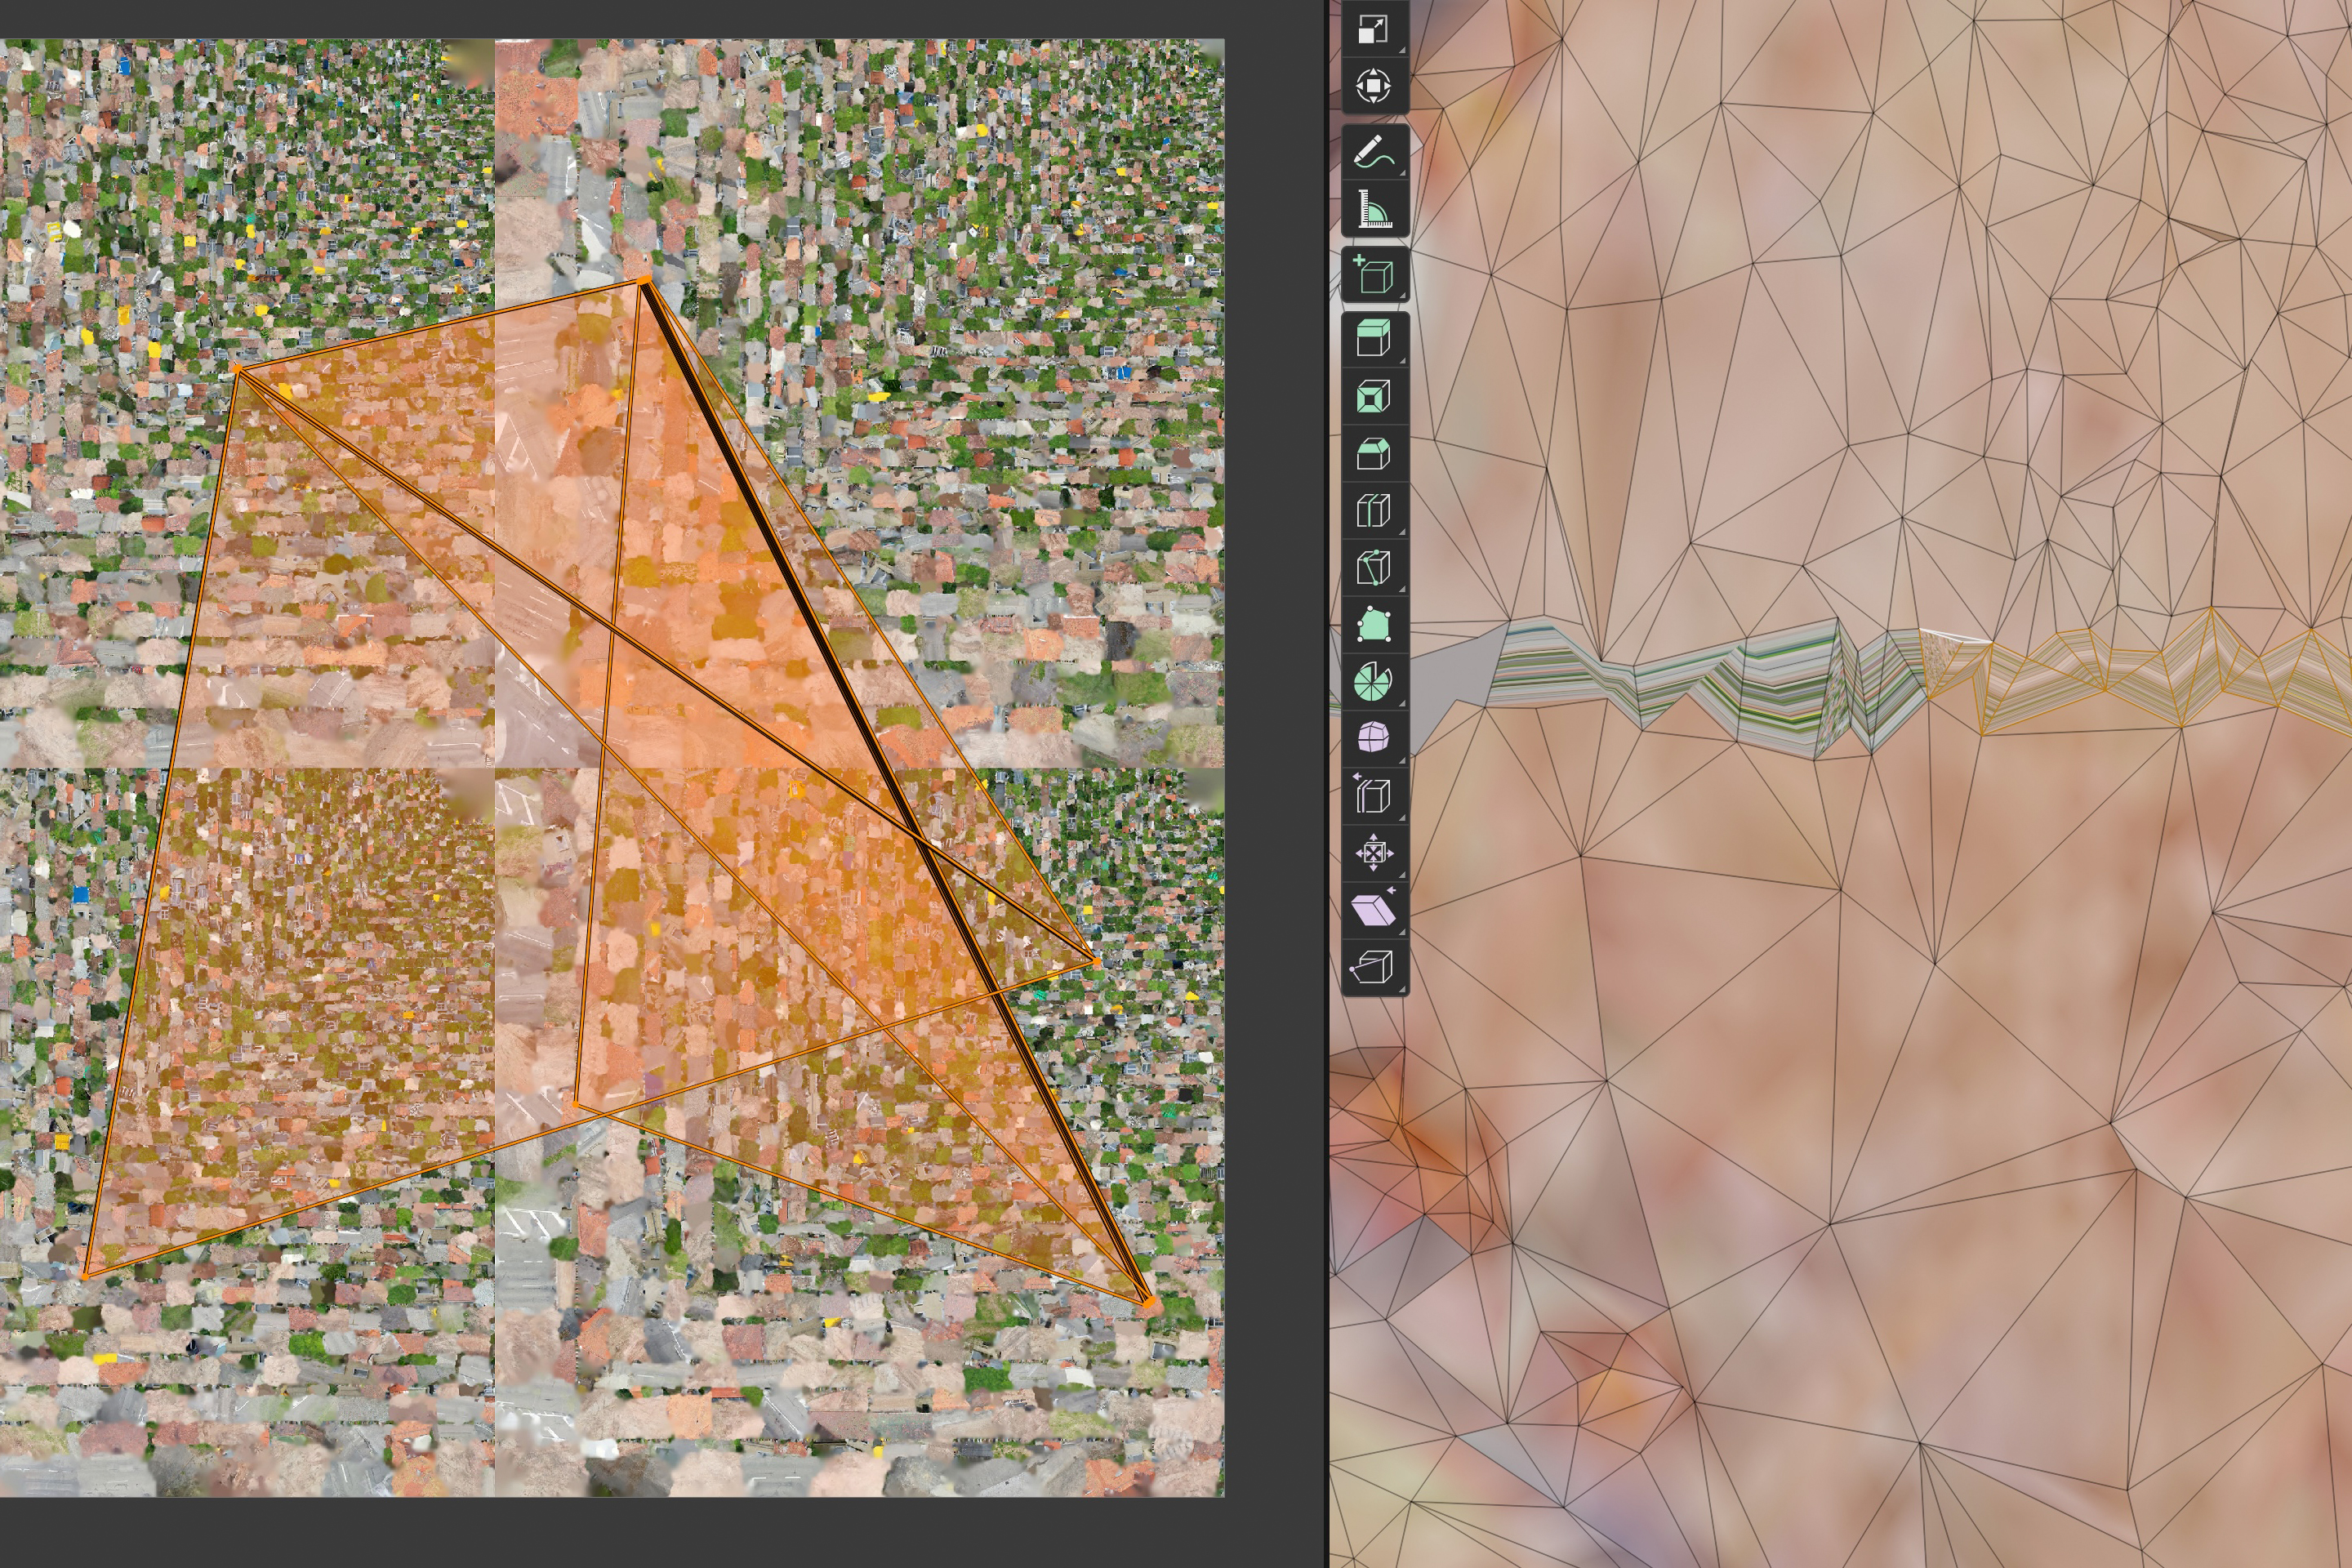
\includegraphics[width=0.4\linewidth]{img/vorbereitungen_blender_modelle/polygone_markieren.jpg}}%
    \qquad
    \subfloat[][]{\includegraphics[width=0.4\linewidth]{img/vorbereitungen_blender_modelle/polygone_textur.jpg}}%
    \caption{Die Polygone werden markiert(a), unwrapped und anschließend auf eine geeignete Fläche auf der Textur gelegt(b).}%
    \label{fig:blender_uv_editing}
\end{figure}

\begin{figure}[hbt!]
    \centering
    \subfloat[][]{\includegraphics[width=0.4\linewidth]{img/vorbereitungen_blender_modelle/blender_vorher.jpg}}%
    \qquad
    \subfloat[][]{\includegraphics[width=0.4\linewidth]{img/vorbereitungen_blender_modelle/blender_nachher.jpg}}%
    \caption{Das Mannschaftsgebäude vor(a) und nach der Bearbeitung(b).}%
    \label{fig:blender_vergleich}
\end{figure}

\subsection{Export und Import}
Damit Unity die 3D Modelle korrekt darstellen kann, werden Anpassungen in Blender vorgenommen:

\begin{itemize}
    \item Vor dem Export werden Texturen in einem Ordner gespeichert. In Blender muss dafür die Option unter \textit{File>External Data>Automatically Pack Resources} ausgeschaltet sein. Anschließend wird mit \textit{File>External Data>Unpack Resources} ein Ordner im Projekt mit den Namen \textit{textures} erstellt, in dem sich die Texturen des Projekts befinden. Nun kann Unity die fehlenden Materials und Texturen im Projekt-Ordner finden,
    \item Unity kann die Texturen nur anwenden, wenn die Textur direkt im \textit{Shader Node} als \textit{Base Color} verbunden ist. Dazwischen befindliche Knoten funktionieren nur in Blender und müssen entfernt werden,
    \item die in Blender genutzten \textit{Modifier}\footnote{https://docs.blender.org/manual/en/latest/modeling/modifiers/index.html} werden angewendet,
    \item damit die Textur korrekt dargestellt werden, werden die Richtungen der \textit{Normalen}\footnote{https://docs.blender.org/manual/en/latest/modeling/meshes/editing/mesh/normals.html?highlight=normals} überprüft, ob diese in die richtige Richtung zeigen. Die Normalen müssen zur korrekten Darstellung nach außen zeigen. In Blender können die Normalen im \textit{Edit Mode} im Viewport Overlay angezeigt und unter \textit{Mesh>Normals} angepasst werden,
    \item Blender und Unity haben unterschiedliche Koordinatensysteme. In Blender zeigt die Z-Achse nach oben und die Y-Achse in die Tiefe, während in Unity die Y-Achse nach oben und die Z-Achse in die Tiefe zeigt. Damit die Modelle aus Blender mit der korrekten Orientierung dargestellt werden, wird das Modell in Blender um -90° gedreht. Mit \textit{STRG + A} und \textit{Rotation} wird die Rotation eingebettet,
    \item beim Export wird das Export-Format \textit{.fbx} benötigt.
\end{itemize}

Jetzt wird das 3D Modell als \textit{.fbx} Datei in Unity importiert. Im \textit{Inspector}-Fenster der \textit{.fbx} Datei werden unter Materials mit \textit{Exctract Materials} Materials in Unity generiert, die die Texturen beinhalten. Der Texturen-Ordner muss im gleichen Ordner liegen. Werden die Texturen nicht gefunden, so können diese händisch in das Projekt eingefügt werden. Um die Texturen den von Unity generierten Materials zu geben, wird im \textit{Inspector} die Textur in das Feld neben \textit{Albedo} eingefügt werden.
% Konzept
% User Interface
% Aufbau der Szenen
% - Menü
% - GPS
% - Standard App
% Implementierung von Features
% - Plane Tracking
% - Occlusion
% - Light Estimation
% Implementierung von Wetter
% - API OpenWeatherMap Anbindung
% - OpenWeatherMap Codes nutzen
% -- States des Wetters
% Lichtsetzung
% - Sonne simulieren
% -- Position der Sonne bestimmen
% -- Farbtemperatur anpassen
% Shader
% - Shatten werfer für den Boden
% - Outline Shader
% - Nass Shader

%KAPITEL 5 Probleme und Lösungen
% GPS Genauigkeit
% - Experiment GPS
% -- GPS Daten vom Vermessungsamt im Vergleich zu Google
% Kompass Genauigkeit
% - Jiggle mit Filter weg
% Mobile Limitierungen
% - Anzahl Polygone der vorhandenen Gebäude
% - Shader -> kein Raytracing
% - Occlusion ohne Tiefensensor


%KAPITEL 6 Future Work
% Sonne nochmal anpassen
% Occlusion mit ARKit testen
% Tiefenkamera verwenden, um Nebel/Dunst zu simulieren
% Blitzeinschläge simulieren
% Partikeleffekte für Schnee (Schnee liegt auf Dach)
% Label mit dem Namen und Infos zum Gebäude in AR
% Benutzung der App als grundlage für andere Projekte
% - Eigene Gebäude reinladen und mit entsprechenden Daten darstellen
% Neumodellierung der Gebäude -> weniger Polygone -> mehr einzelne Materialien, die angepasst werden können

%KAPITEL Fazit

% ANHANG
% UML Klassen Auflistung

\include{content/figures}       % Example figures
\include{framework/figures}     % List of figures, bibliography
\include{framework/affirmation} % Eidesstattliche Erklärung 
\printbibliography
\end{document}